\chapter{Langlands纲领的几何重述之三：Hecke代数}\label{L12}\lecturedate{2020/03/25}\sourcepage{98}
在此前见过的Langlands对应中，Hecke代数和Hecke特征函数都起着关键作用。在球面情形，对应按以下方式建立：
\begin{figure}[H]\centering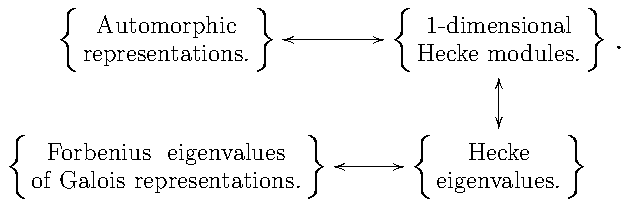
\includegraphics[width=0.5071\paperwidth]{images/L12-p098-correspondence.pdf}\end{figure}
先回顾关于Hecke代数的一个基本事实。设$F$为非阿基米德局部域，$K$为$G=\GL_n(F)$的紧开子群。与$K$相关的Hecke代数$\mathcal H_K$，是$G$上所有紧支函数$\phi$组成的向量空间，其中对任意$h_1,h_2\in K$，有$\phi(h_1gh_2)=\phi(g)$；其环结构为
\[(\phi*\psi)(g)=\int_G\phi(gx^{-1})\psi(x)\,dx,\]
其中$dx$为Haar测度。

设$\pi:G\to\GL(V)$为复向量空间$V$上的表示，$V$可能是无限维的。若对每个$0\ne v\in V$，稳定子群$G^v:=\{g\in G\mid\pi(g)v=v\}$均为开子群，则称表示\textbf{光滑}。对光滑表示$(\pi,V)$，可定义同态$\pi:\mathcal H_K\to\End(V)$：
\[\pi(\phi)v=\int_G\phi(g)\pi(g)v\,dg.\]
\sourcepage{99}
回忆：若$(\pi,V)$光滑，且对每个紧开子群$K'$，$V^{K'}$都有限维，则称它\textbf{可容许}。于是有如下定理。
\originalnumber{1}
\begin{theorem}\label{L12S0O1}
\begin{enumerate}[label=(\roman*)]
\item 若$(\pi,V)$为不可约可容许表示，且$V^K\ne0$，则$V^K$为不可约，即单的$\mathcal H_K$模。
\item 若$(\pi,V)$和$(\sigma,W)$为不可约可容许表示，且$V^K,W^K$非零并作为$\mathcal H_K$模同构，则$\pi$与$\sigma$等价。
\end{enumerate}
\end{theorem}
\begin{proof}[结论(i)的证明概要]
由于$G$全不连通且局部紧，其单位元有由紧开子群组成的邻域基。取$0\ne u\in V^K$，需要证明：对任意$v\in V^K$，存在$\phi\in\mathcal H_K$，使$\pi(\phi)u=v$。由不可约性，可写$v=\sum_ja_j\pi(g_j)u$。对每个$g=g_j$，令$K_0=gKg^{-1}\cap K$。它仍为$G$的紧开子群；由于$K$紧，$K_0$在$K$中的指数有限。于是
\[KgK=\bigsqcup_{j=1}^{N}\gamma_jgK,\]
其中$\gamma_j$为$K/K_0$的陪集代表；$KgK$具有有限测度。设$\phi_g=\operatorname{vol}(KgK)^{-1}\mathbf1_{KgK}$，其中$\mathbf1_S$为$S$的示性函数。则$\pi(\phi_g)u$是$\pi(g)u$的左$K$平均。对$v$的上述线性组合取平均，由$v\in V^K$，便有$\pi(\sum_ja_j\phi_{g_j})u=v$。
\end{proof}
\begin{proof}[结论(ii)的证明思路]
从给定的$\mathcal H_K$模同构$V^K\xrightarrow{\sim}W^K$，构造$\mathcal H$模同构$V\xrightarrow{\sim}W$，其中$\mathcal H$为$G$上局部常值紧支函数组成的卷积代数。随后这一同构也是$G$模同构：若$K_v$为包含于$G^v$的紧开子群，则对$\phi=\operatorname{vol}(K_v)^{-1}\mathbf1_{gK_v}$，有$\pi(g)v=\pi(\phi)v$。
\end{proof}
\section{几何情形中的Hecke代数}\label{L12S1}\idx{球面Hecke代数}
设$X$为完备光滑曲线，函数域为$F$。对每个素位$x\in|X|$，局部Hecke代数$\mathcal H(\GL_n(F_x),\GL_n(\OO_x))$与紧子群$\GL_n(\OO_x)$相关，亦称\textbf{球面Hecke代数}。它是交换的，并且几乎是一个多项式代数。更精确地，
\[\mathcal H(\GL_n(F_x),\GL_n(\OO_x))=\C[T_x^1,\ldots,T_x^{n-1},T_x^n,(T_x^n)^{-1}].\]
\sourcepage{100}
其中，$T_x^i$是对角矩阵
\[g_i=\operatorname{diag}(\underbrace{\omega_x,\ldots,\omega_x}_{i\text{次}},1,\ldots,1)\]
的$\GL_n(\OO_x)$双陪集的示性函数；$\omega_x$为$\OO_x$的素元，即$\ord_{\p_x}(\omega_x)=1$。换言之，$T_x^i=\mathbf1_{\GL_n(\OO_x)g_i\GL_n(\OO_x)}$。

还定义整体Hecke代数
\[\mathcal H(\GL_n(\A_F),K):=\bigotimes_{x\in|X|}'\mathcal H(\GL_n(F_x),\GL_n(\OO_x)),\]
其中照例$K=\prod_{x\in|X|}\GL_n(\OO_x)$是$\GL_n(\A_F)$的最大紧子群。它作用于$\mathcal A_0(G)^K$，即双商
\[\GL_n(F)\backslash\GL_n(\A_F)/K\]
上的尖点自守函数空间。

希望以几何语言解释Hecke算子。回忆，作为集合，$\GL_n(F)\backslash\GL_n(\A_F)/K\cong\operatorname{Bun}_n(X)$的同构类集合。因此，要在$\operatorname{Bun}_n(X)$上描述Hecke代数作用。先从集合论解释。记$\mathcal H_x^i$为数据$(\mathcal M,\mathcal M',\beta)$的同构类集合，其中$\mathcal M,\mathcal M'$为$X$上的秩$n$向量丛，$\beta:\mathcal M\hookrightarrow\mathcal M'$为嵌入，商$\mathcal M'/\mathcal M$支于$x$，被$x$的极大理想消去，且长度为$i$。记$k_x$为$x$的剩余域，则有
\begin{equation}\tag{1.1}\label{L12eq11}
\begin{aligned}
0\to\ker(\beta\otimes k_x)\to\mathcal M\otimes k_x\xrightarrow{\beta\otimes k_x}\mathcal M'\otimes k_x\\
\longrightarrow(\mathcal M'/\mathcal M)\otimes k_x\to0.
\end{aligned}
\end{equation}
其中$\ker(\beta\otimes k_x)\cong\operatorname{Tor}^{\OO_{X,x}}_1(\mathcal M'/\mathcal M,k_x)$，且$\beta\otimes k_x$的核与余核都非典范地同构于$k_x^i$。

从$\mathcal H_x^i$到$\operatorname{Bun}_n(X)$有两个映射$h^\leftarrow,h^\rightarrow$\znote{Hecke对应是向量丛模叠之间的一类对应：对每个 $i$ 与 $x\in X$，把「$\mathcal M\hookrightarrow\mathcal M'$ 且商 $\mathcal M'/\mathcal M$ 支于 $x$、长度为 $i$」的数据汇成叠 $\mathcal H_x^i$，即得对应 $\operatorname{Bun}_n(X)\xleftarrow{h^\leftarrow}\mathcal H_x^i\xrightarrow{h^\rightarrow}\operatorname{Bun}_n(X)$，其纤维是Grassmann簇。由它给出的积分变换 $(h^\rightarrow)_*(h^\leftarrow)^*$ 称为Hecke变换，在函数层面就是Hecke算子。要点是：Hecke算子并非两个函子的复合，而是「先拉回、再沿对应纤维积分」的对应运算。[来源：nLab "Hecke correspondence"，\url{https://ncatlab.org/nlab/show/Hecke+correspondence}（Last revised 2026-09-07；2026-11-14 访问）。]}，定义如下：
\begin{figure}[H]\centering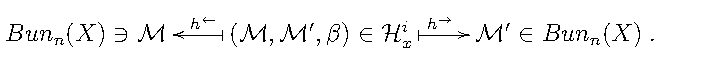
\includegraphics[width=0.5687\paperwidth]{images/L12-p100-Hecke.pdf}\end{figure}
$h^\leftarrow$的纤维典范地等同于Grassmann簇$\operatorname{Gr}(\mathcal M\otimes k_x,i)$的$k_x$点集；$h^\rightarrow$的纤维则等同于$\operatorname{Gr}(\mathcal M'\otimes k_x,n-i)$的$k_x$点集。记$\operatorname{Funct}(\operatorname{Bun}_n(X))$为其同构类上的函数空间，则有算子$(h^\rightarrow)_*(h^\leftarrow)^*$；下标$*$表示沿纤维积分，上标$*$表示拉回。
\sourcepage{101}
\originalnumber{1}
\begin{proposition}\label{L12S1O1}
算子$(h^\rightarrow)_*(h^\leftarrow)^*$等于局部Hecke代数$\mathcal H(\GL_n(F_x),\GL_n(\OO_x))$中的$T_x^i$。
\end{proposition}
把各个$\mathcal H_x^i$合在一起，得到$\mathcal H^i:=\bigcup_{x\in|X|}\mathcal H_x^i$，并有以下三个映射：
\begin{figure}[H]\centering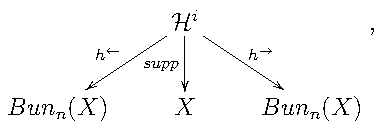
\includegraphics[width=0.3091\paperwidth]{images/L12-p101-support.pdf}\end{figure}
$\operatorname{supp}$在$x\in X$处的纤维为$\mathcal H_x^i$。

也可以用几何语言表达尖点性。取分拆$n=n_1+n_2$，考虑下列短正合列的同构类集合$\operatorname{Flag}_{n_1,n_2}^n$：
\[0\to\mathcal M_1\to\mathcal M\to\mathcal M_2\to0,\]
其中$\mathcal M_1,\mathcal M_2$分别为秩$n_1,n_2$的向量丛。有
\begin{figure}[H]\centering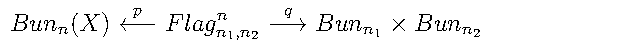
\includegraphics[width=0.5141\paperwidth]{images/L12-p101-flag.pdf}\end{figure}
这两个映射分别将短正合列送到$\mathcal M$和$(\mathcal M_1,\mathcal M_2)$。于是有
\[q_*p^*:\operatorname{Funct}(\operatorname{Bun}_n(X))\to\operatorname{Funct}(\operatorname{Bun}_{n_1}(X)\times\operatorname{Bun}_{n_2}(X)).\]
函数$f$具有尖点性，当且仅当对所有满足$n_1+n_2=n$的正整数$n_1,n_2$，都有$q_*p^*(f)=0$。然而，几何情形中用来解释自守表示的实际对象，是反常层，而不是函数。
\section{从函数到层}\label{L12S2}\idx{层与函数的对应}\idx{反常层}
先设$V$为$\F_q$上的代数簇，$Y=V(\F_q)$为其$\F_q$点集，$\mathcal F$为$V$上的$\ell$进$\overline{\Q}_\ell$层。对$x\in Y$上方的几何点$\overline x$，
\sourcepage{102}
茎$\mathcal F_{\overline x}$为$\overline{\Q}_\ell$向量空间，并带有$\Gal(\overline{k_x}/k_x)=\Gal(\overline{\F}_q/\F_q)$的自然作用，给出同态$\rho_x:\Gal(\overline{k_x}/k_x)\to\GL(\mathcal F_{\overline x})$。几何Frobenius元素$\mathrm{Fr}_x$拓扑生成这一Galois群。因此可在$Y$上定义函数
\begin{equation}\tag{2.1}\label{L12eq21}
f_{\mathcal F}:Y\to\overline{\Q}_\ell,\qquad f_{\mathcal F}(x)=\Tr(\rho_x(\mathrm{Fr}_x)).
\end{equation}
\originalnumber{1}
\begin{note}[L12S2O1]
一个$\ell$进$\overline{\Q}_\ell$层$\mathcal F$可以在某个$\Q_\ell$的有限扩张$E$上定义：取其整数环$\OO_E$上的$\ell$进层$\mathcal F_{\OO_E}$，形式地与$\overline{\Q}_\ell$张量。相应平展上同调为
\[H^r_{\mathrm{ét}}(\mathcal F)=H^r_{\mathrm{ét}}(\mathcal F_{\OO_E})\otimes_{\OO_E}\overline{\Q}_\ell,\]
因而是$\overline{\Q}_\ell$向量空间。
\end{note}
% [Tutor Note: 原书 p102 的 Remark 2.1 把 $\overline{\Q}_\ell$ 层说成「$\Z_\ell$ 层形式张量 $\Q_\ell$」，上同调也写作 $\otimes_{\Z_\ell}\Q_\ell$；译文按通行定义改为取某个 $\Q_\ell$ 的有限扩张 $E$，用其整数环 $\OO_E$ 上的层与 $\overline{\Q}_\ell$ 张量。]
\eqref{L12eq21}中的函数定义可以推广到$\ell$进层复形。设$\mathcal K^\bullet$为这样的复形，则$\Gal(\overline{k_x}/k_x)$作用于上同调层$\mathcal H^i(\mathcal K^\bullet)$在$\overline x$处的茎。定义
\begin{equation}\tag{2.2}\label{L12eq22}
f_{\mathcal K^\bullet}(x):=\sum_i(-1)^i\Tr(\mathrm{Fr}_x\mid\mathcal H^i(\mathcal K^\bullet)_{\overline x}).
\end{equation}
\eqref{L12eq22}提示，可以使用有界可构造导出范畴$D^b_c(V)$中的对象，而不只使用层。然而，$D^b_c(V)$并非阿贝尔范畴。适当的选择是反常层范畴：反常层并非通常意义的层，而是满足其茎与余茎上同调非零次数限制的$\ell$进层复形。

已经说明了$\F_q$上的代数簇中函数与层的关系。对$\C$上的代数簇，反常层的概念也完全有意义。此外，还可以进一步将反常层重述为$\mathcal D$模。后续各讲将详细介绍反常层和$\mathcal D$模。

现在的问题是：如何在$\operatorname{Bun}_n(X)$上定义层，乃至导出范畴$D^b_c(\operatorname{Bun}_n(X))$？$n=1$时，次数0线丛的刚性化模问题由代数概形$\operatorname{Jac}(X)$表示。一般地，$\operatorname{Bun}_n(X)$只是代数叠。

要在叠上定义层，可以从概形转向函子。如上一讲所述，每个$k$概形$S$都关联反变函子$\underline S:(\mathrm{Sch}/k)\to\mathrm{Sets}$，$T\mapsto\Hom(T,S)$。
\sourcepage{103}
由Yoneda引理，概形由其函子完全确定。叠$\mathfrak X$也是函子，且$\Hom(\underline S,\mathfrak X)$为范畴$\mathfrak X(S)$。在$\mathfrak X$上定义$\ell$进层，是给每个对象$\eta\in\mathfrak X(S)$赋予$S$上的$\ell$进层，并给每个箭头赋予层之间的同构，同时要求这些数据与基变换相容。于是，$D^b_c(\mathfrak X)$也有意义。特别地，$\mathfrak X$的$\F_q$点实际构成范畴$\mathfrak X(\Spec\F_q)$；每个$\mathcal F\in D^b_c(\mathfrak X)$都给出其对象同构类上的函数$f_{\mathcal F}$。

现在把$\operatorname{Bun}_n(X)$看成代数叠。$\mathcal H_x^i$、$\mathcal H^i$也具有叠结构。因此，$h^\leftarrow,h^\rightarrow$是叠之间的态射，其纤维为概形形式的Grassmann簇。它们可表示，所以可以讨论相应的拉回和推前。定义Hecke函子
\[T_x^i:D^b_c(\operatorname{Bun}_n(X))\to D^b_c(\operatorname{Bun}_n(X)),\]
由
\[\mathcal K^\bullet\longmapsto(h^\rightarrow)_*(h^\leftarrow)^*(\mathcal K^\bullet)[i(n-i)]\]
给出。上下标$*$在这里均指导出函子；方括号表示上同调平移（Tate 平移）。

还定义Hecke函子$T^i:D^b_c(\operatorname{Bun}_n(X))\to D^b_c(X\times\operatorname{Bun}_n(X))$：
\[\mathcal K^\bullet\longmapsto(\operatorname{supp}\times h^\rightarrow)_*(h^\leftarrow)^*(\mathcal K^\bullet)[i(n-i)].\]
\idx{Hecke函子}
\section{Langlands对应的几何表述}\label{L12S3}\idx{几何Langlands对应}\idx{Hecke特征层}
在几何Langlands猜想\znote{几何Langlands对应是经典Langlands对应的几何化：Galois表示一侧换成曲线 $X$ 上的局部系统，自守表示一侧换成 $\operatorname{Bun}_n(X)$ 上的反常层（Hecke特征层），并在两者之间建立函子性的对应。与经典情形给出「表示的对应」不同，几何版本预期是范畴层面的对应：平坦联络的局部系统与 $\operatorname{Bun}_n(X)$ 上的反常层（或相应范畴中的对象）应当互相对应；本讲只陈述其中单向的构造，即由局部系统造出Hecke特征层。[来源：nLab "Langlands program"，\url{https://ncatlab.org/nlab/show/Langlands+program}（Last revised 2024-03-28；2026-11-14 访问）。]}中，以曲线$X$上的$n$维局部系统替代经典理论中的Galois表示；在自守一侧，则使用叠$\operatorname{Bun}_n(X)$上的反常层，即Hecke特征层。这里的几何Langlands对应按从局部系统到Hecke特征层的单向映射表述，因为Hecke特征层是相对于局部系统定义的。

设$E=E_\sigma$为$X$上的$\overline{\Q}_\ell$局部系统，对应表示
\sourcepage{104}
$\sigma:\widehat\pi_1(X)\to\GL_n(\overline{\Q}_\ell)$。若对每个$i=1,\ldots,n$，存在同构
\[T^i(\mathcal F_\sigma)\cong\bigwedge^iE_\sigma\boxtimes\mathcal F_\sigma,\]
则称$\mathcal F_\sigma\in D^b_c(\operatorname{Bun}_n(X))$为相对于$\sigma$的\textbf{Hecke特征层}\znote{Hecke特征层是Hecke变换的本征对象：要求对每个 $i$ 都有 $T^i(\mathcal F_\sigma)\cong\bigwedge^iE_\sigma\boxtimes\mathcal F_\sigma$，即Hecke变换把 $\mathcal F_\sigma$ 送到自身的「张量倍数」，倍数由局部系统 $E_\sigma$ 的外幂丛 $\bigwedge^iE_\sigma$ 给出。这与经典理论中Hecke特征函数的地位平行：自守表示被Hecke算子作用后仍是自身的倍数，倍数即Hecke本征值；几何化之后本征值由外幂丛取代。注意 eigensheaf 是按定义相对于某个局部系统而言的，故几何Langlands对应只能是单向的映射。[来源：nLab "Hecke eigensheaf"，\url{https://ncatlab.org/nlab/show/Hecke+eigensheaf}（该条目较短且未标注 Last revised，2026-11-14 访问；另参 "Hecke correspondence"）。]}；其中$\bigwedge^i$表示第$i$次外幂。

几何Langlands对应由以下定理表述。
\originalnumber{1}
\begin{theorem}\label{L12S3O1}
设$X$为定义在$\F_q$或$\C$上的光滑完备曲线。对$X$上的每个不可约秩$n$局部系统$E$，都存在反常层$\mathcal F_\sigma\in D^b_c(\operatorname{Bun}_n(X))$，它是相对于$E$的Hecke特征层，并自动具有尖点性。此外，在每个参数化秩$n$、次数$d$向量丛的连通分量$\operatorname{Bun}_n^d(X)$上，$\mathcal F_\sigma$不可约。
\end{theorem}
换言之，这一几何表述断言存在如下单向对应：
\begin{figure}[H]\centering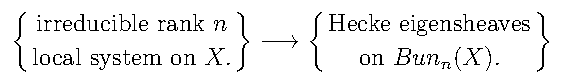
\includegraphics[width=0.4549\paperwidth]{images/L12-p104-correspondence.pdf}\end{figure}
\originalnumber{2}
\begin{note}[L12S3O2]
这里在Galois一侧只考虑处处非分歧表示，在自守一侧只考虑所有局部分量$\pi_x$均为球面表示的$\pi=\bigotimes_x'\pi_x$。而经典Langlands纲领中的Galois表示仅要求几乎处处非分歧，自守表示也仅要求几乎处处球面。在允许有限多个素位处分歧的更一般几何情形中，也有一些结果，但本课程不讨论它们。
\end{note}
\needspace{5\baselineskip}\section{第12讲参考文献}\label{L12S4}
\begin{references}
\refitem{L12bibBG}{BG} J. Bernstein and S. Gelbart, eds, \emph{An introduction to the Langlands Program}, Birkhäuser, 2004, Chapter 12 written by D. Gaitsgory.
\end{references}
